%\documentclass[draft]{acm_proc_article-sp}
\documentclass{acm_proc_article-sp}

\graphicspath{{../figures/}}
\begin{document}

\title{OpenCUDA+MPI: A Framework for Heterogeneous GP-GPU Computing}
\subtitle{[Extended Abstract]}
\numberofauthors{3}
\author{
% 1st. author
\alignauthor
Kenny Ballou\\
    \affaddr{Boise State University}\\
    \affaddr{Dept. of Computer Science}\\
    \affaddr{1910 University Dr.}\\
    \affaddr{Boise, Idaho, USA}\\
    \affaddr{kennyballou@boisestate.edu}\\
% 2nd. author
\alignauthor
Nilab Mohammad Mousa\\
    \affaddr{Boise State University}\\
    \affaddr{Dept. of Computer Science}\\
    \affaddr{1910 University Dr.}\\
    \affaddr{Boise, Idaho, USA}\\
    \affaddr{nmousa@onyx.boisestate.edu}\\
% 3rd. author
\alignauthor
Alark Joshi, PhD.\\
    \affaddr{Boise State University}\\
    \affaddr{Dept. of Computer Science}\\
    \affaddr{1910 University Dr.}\\
    \affaddr{Boise, Idaho, USA}\\
    \affaddr{alarkjoshi@boisestate.edu}\\
}
\date{30 July 1999}
\maketitle{}
\begin{abstract}

The introduction and rise of General Purpose Graphics Computing has
significantly impacted parallel and high performance computing. It has
introduced challenges when it comes to distributed computing with GPUs. Current
solutions target specifics: specific hardware, specific network topology, a
specific level of processing.  Those restrictions on GPU computing limit
scientists and researchers in various ways. The goal of OpenCUDA+MPI project is
to develop a framework that allows researchers and scientists to write a
general algorithm without the overhead of worrying about the specifics of the
hardware and the cluster it will run against while taking full advantage of
parallel and distributed computing on GPUs. As work toward the solution
continues to progress, we have proven the need for the framework and expect to
find the framework enables scientists to focus on their research.

\end{abstract}

% A category with the (minimum) three required fields
\category{D.3.3}{Software}{Language Constructs and Features -\\{}
Frameworks}[Modules, Packages]

\terms{Software Libraries, Frameworks}

\keywords{Parallel and Distributed Computing, High-Performance\\{} Computing,
Software Libraries, Frameworks}

\section{Introduction}

Increasingly, graphics processing units are being used for general purpose
computation. They have significantly altered the way high performance
computing tasks can be performed today. Many scientific applications require a
large number of floating point number operations. CPU's are not sufficient to
carry out such computationally intensive tasks.  \texttt{CUDA} utilizes the
power of \texttt{GPUs} to achieve dramatic increases in computing performance
\cite{website:cudaCProgrammingGuide}. Distributing work with MPI can increase
the performance of CPU's. Combined with \texttt{CUDA}/ \texttt{GPU's}, the
performance increase can be even greater.  However, developing the codes
required for this can be very expensive and difficult to get correct.
\texttt{OpenCUDA+MPI} attempts to solve these issues.

\subsection{Project Objectives}

We have several goals we want to accomplish in creating \texttt{OpenCUDA+MPI}.
Namely, the framework itself, a collection of related administration tools and
configurations, and once a stable version of the framework is finished, it is
released as Free and Open-Source software.

\section{Methodology}

To fully understand the purpose of creating a framework, we first set out to
attempt developing parallel code \emph{without} our proposed framework.

We also want to not only compare times of development speed, but actual running
time of each solution. As such, we developed a CPU only, a single GPU, and a
distributed GPU solution to the N-Body problem and compared running times of
each for several different problem sizes.

The N-Body problem was chosen as a test problem because it is \emph{not} an
embarrassingly parallel problem and, as such, requires inter-communication.

\section{Results}

We were able to show that distributing work over a cluster can significantly
decrease the amount of time required for a problem. For example, processing the
N-Body problem for 200 thousand bodies on a single CPU required $114349$
seconds (about 31 hours), as compared to a single GPU which required $52$
seconds and distributing over 16 GPU's only took $21$ seconds. [Currently, a
comparison between the distributed code with and without the framework is not
available.]

Although biased, it was interesting to notice the development time difference
between writing the distributed code without the framework as compared to with
the framework. Namely, without the framework, it required several weeks,
whereas, with the framework, it required less than a week.

\begin{figure}
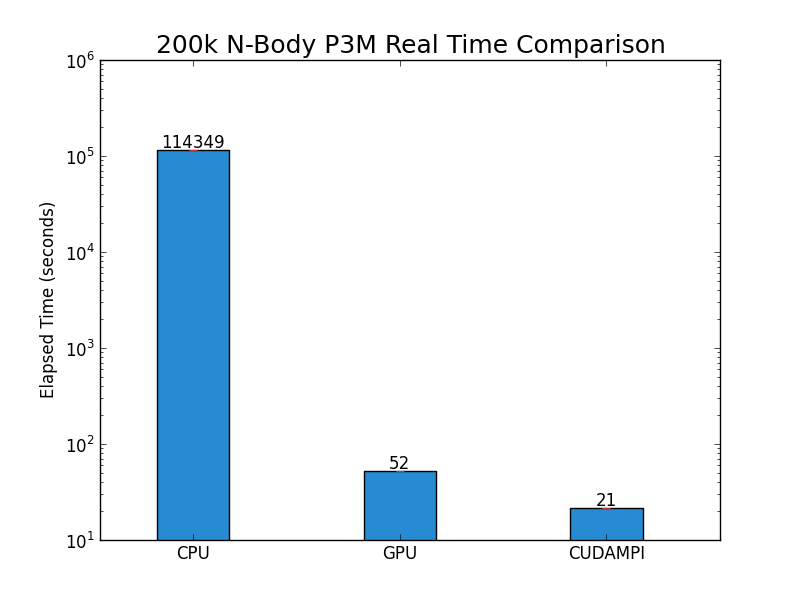
\includegraphics[scale=0.4]{200k_bar_chart.png}
\caption{200k N-Body P3M Time Comparisons}
\end{figure}

\begin{figure}
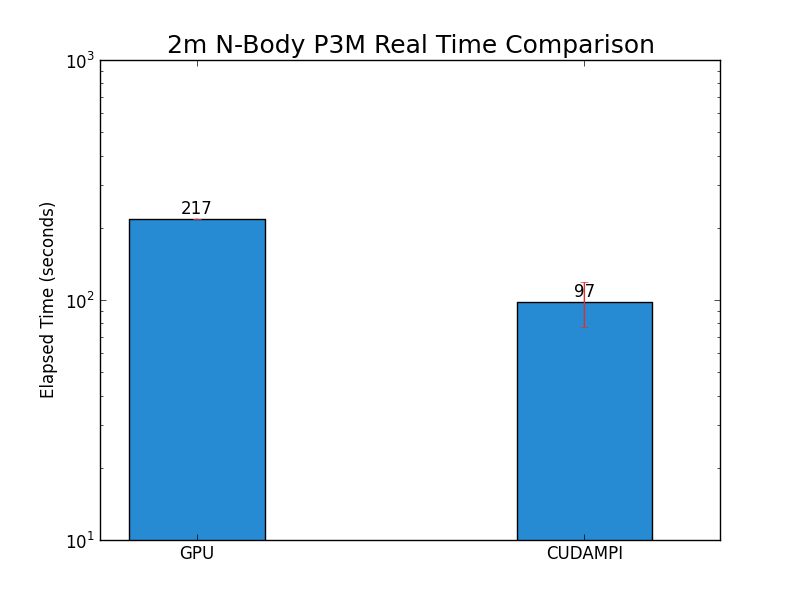
\includegraphics[scale=0.4]{2m_bar_chart.png}
\caption{2m N-Body P3M Time Comparisons}
\end{figure}

\begin{figure}
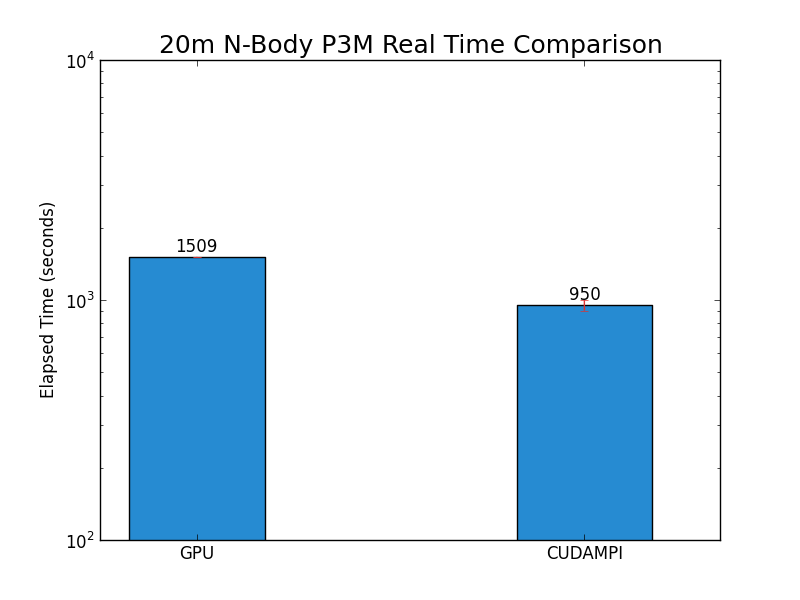
\includegraphics[scale=0.4]{20m_bar_chart.png}
\caption{20m N-Body P3M Time Comparisons}
\end{figure}

\section{Conclusions}

We can clearly see the increase in performance when we distribute our work over
many machines. If our problem is particularly I/O bound, however, we may be
causing more slow downs or bottlenecks than worth the computational performance
increase.

We need to test the framework more, and with more, different problems. Doing so
would highlight areas that need adjustment or re-working. Further, it would
show the framework's viability to others and in other problem spaces.

\section{Future Work}

As we continue to work on the framework, there are a few more features and
goals that we wish to achieve. Namely, we would like to add better debugging,
logging, and profiling functionality, expose control of \texttt{CUDA} device
initialization, add automatic/ configurable check pointing, and finish up node
administration and configuration.

\section{Acknowledgments}

We would like to give a special thanks to Boise State University's Student
Research Initiative program and program director: Liljana Babinkostova, PhD.
without whom, this project never would have been possible. We would also like
to give an extra special thanks to our mentor: Alark Joshi, PhD.

\bibliographystyle{abbrv}
\begin{thebibliography}{4}
\bibitem{website:cudaCProgrammingGuide}
CUDA C Programming Guide. May 2013.\\{}
\bibitem{website:openmpi}
{Open MPI}. http://www.open-mpi.org/, 2013.\\{}
\bibitem{website:whatcuda}
What is {CUDA}.
https://developer.nvidia.com/what-cuda, 2013.\\{}
\bibitem{website:pycuda}
Andreas Kloechner. PyCUDA Documentation, 2008.\\{}
\end{thebibliography}

\balancecolumns{}
\end{document}
